
% no longer than 5 pages including figures and tables + as many pages as needed for references
% 2 columns on 8.5 x 11 inch paper
% 10 point Times Roman font on 12 point single spaced leading, 1 inch margins
% 0.25 inch gutter (seeparation between columns)

% Title, author names, affiliations, abstract should appear on first page
% pages should be numbered
% figures and tables should not require magnification, may contain color but should be
% legible in black and white

\documentclass[sigplan,10pt,review,authorversion]{acmart}\settopmatter{printfolios=true,printccs=false,printacmref=false}

\citestyle{acmnumeric}

% REMOVE FOR ACCEPTED
\renewcommand\footnotetextcopyrightpermission[1]{} % removes footnote with conference information in first column
%\pagestyle{plain}

\expandafter\let\csname not=\endcsname\relax
\expandafter\let\csname not<\endcsname\relax
\expandafter\let\csname not>\endcsname\relax

\RequirePackage{pdf14}
\usepackage{unicode-math}

\usepackage{balance}
%% \usepackage{fixltx2e} % travis-ci has an old version of latex and needs this for \textsubscript, etc
\usepackage{mdframed}
%% \usepackage{booktabs}
%% \usepackage{enumitem}
%% \usepackage{amsmath}
%% \usepackage{amsthm}
%% \usepackage{color}
%% \usepackage{calc}
\usepackage{xspace}
%% \usepackage{upgreek}
\usepackage{graphicx}
%% \usepackage{natbib}
%% \usepackage{alltt}
\usepackage{fancyvrb}
%\usepackage{array}
%% \usepackage{tabu}
%% \usepackage{multirow}
\usepackage{mathpartir}
%% \usepackage{balance}
\usepackage{subcaption}
\usepackage{wrapfig}
%% \usepackage{framed}
\usepackage{colortbl}
\usepackage{tikz}
\usetikzlibrary{decorations.markings}
\usetikzlibrary{arrows,shapes}
\usetikzlibrary{positioning}
\tikzset{
    >=stealth,
    %auto,
    %node distance=3.5cm,
    font=\scriptsize,
    ack/.style={align=center,ellipse,draw},%circle,draw,thick,align=center},
    minimum size=20pt
}
\usepackage{multicol}
\usepackage{pgfplots}\pgfplotsset{compat=1.13}


%% Requires:
%% \usepackage{color}
%% \usepackage{calc}
%% \usepackage{xspace}
\usepackage{pifont}

\usepackage{tikz-cd}

%% \usepackage{upgreek}

% \usepackage{MnSymbol}

\setlength{\bibsep}{1pt}

%\newtheorem{theorem}{Theorem}
%\newtheorem{lemma}{Lemma}
%\newtheorem{definition}{Definition}

\definecolor{gray}{rgb}{0.9,0.9,0.9}
\definecolor{red}{rgb}{1,0,0}
\newcommand{\graybox}[1]{\mbox{\setlength{\fboxsep}{0.5pt}%
    \colorbox{gray}{$#1$}}}

%\newcommand{\graybox}[1]{#1}

\newcommand{\var}[1]{\mathit{#1}}

\newcommand{\fixme}[1][\relax]{{\color{red}{FIXME: #1}}}


\newcommand{\ma}[1]{\ensuremath{#1}\xspace}


\title{Four reasons your build is slow}
\author{Sarah Spall}
\affiliation{Indiana University}
\author{Sam Tobin-Hochstadt}
\affiliation{Indiana University}


\begin{abstract}
Spending time waiting for code to compile is cliche enough to be
featured in XKCD, yet it continues to plague software
developers. Fortunately, software builds are an embarassingly parallel
problem, and so we can finally make use of all those extra cores---a
happy coincidence of software complexity and hardware trends.

Unfortunately, the story is not quite this rosy, as almost anyone who
waits for software to build knows. Real build systems fail to be the
embarassingly parallel poster child we hope for, and instead are slow
in a wide variety of ways.

To investigate this problem, we have built an automated build analysis
tool that works for arbitrary build systems using the venerable
\texttt{make} tool. Our analysis can predict parallel speedup, analyze
the long pole of dependencies, determine false dependencies, and
predict parallelism in a perfect world. We use our tool on real-world
project to describe four problems found in actual software builds, and
in some cases how to fix them.
\end{abstract}


\begin{document}

\maketitle

\section{Introduction}

\begin{Verbatim}[commandchars=\\\{\},codes={\catcode`$=3\catcode`^=7\catcode`_=8},fontsize=\small,numbers=left,xleftmargin=5mm]
all:
  cc in.c -o out.o
\end{Verbatim}
  


\section{Analysis tool}
\label{sec:analysis}
In this section we describe the tools we use to analyse, diagnose problems, and suggest solutions
for project builds that use make.  In section \ref{sec:makeanalysis} we will discuss how we use
a modified version of GNU Make to record enough information about a project's build to later
reconstruct the build graph during a post mortem analysis.  In section \ref{sec:straceinstr} we
will discuss how we additionally use a slightly modified version of strace to record all of the
system calls made during the build and then use this information to determine the real dependencies
of the build by looking at which files were actually touched. In section \ref{sec:revisegraphs} we
will look at how we combine the information from these two tools to transform build graphs into
new graphs with potentially more parallelism and provide insight into the build graph's structure.
% what else to say here?

\subsection{Make analysis and instrumentation}
\label{sec:makeanalysis}

To collect the desired level of information from a run of GNU Make \cite{}, we run make with the
debug level of 'verbose', use our own make wrappers which print additional information, and use
a modified version of make which prints directory and timing information for each shell command
it runs.  All of this information is written to a file and is used by our tool to reconstruct
the build graph after the build successfully completes.  We are able to re-construct a graph which
contains all of the shell commands executed to build the project as well as the time it took
to execute each one.  With this timing information we can calculate the work and the span of the
build.  The work is the total time to execute every shell command in the build graph.  The span is
the longest time to execute any sequence of shell commands in the build graph which must be
executed sequentially.  For example: the span of a make rule is the longest time to execute a
dependency plus the sum of the times to execute each recipe.  And parallelism is defined to be
span/work, therefore to increase the parallelism of a project and reduce the overall running time,
the span must be decreased.

Identifying the span path in the build allows the user to target the most appropriate place
for performance improvements.  In section \ref{} we will discuss some projects that were analysed
using this tool and what we learned about their parallelism and how to improve it.

% Have a wrapper around gnu make; which prints information about which top-level make
% is being invocated and prints out the directory; this wrapper also times the call to
% actual gnu make

% have a 2nd wrapper around gnu make; which is called for ``sub makes''. we tell actual
% make that we want it to call this for all $(MAKE) calls in the makefile.  this wrapper
% similarly to the top-make wrapper prints out which make is being executed as well as the
% directory and time of the actual make call.
% WHY do we need the above information??

% The most important change is in make itself; where we modified make to print each shell
% command it is running as well as the time the shell command took.
% this data lets us calculate the work and the span of the build and lets us attribute span
% to the correct targets and shell commands.
% Since we are able to store the command run by make in the reconstructed build graph we can
% rerun those ocmmands to replay the build; and it didn't require us to parse the makefile
% ourselves.

% tool can calculate work and span of the build and attribute the span to the correct nodes
% so that the user can focus their performance improvements on the portiosn of the graph that
% will have the most affect.

\subsection{Strace instrumentation}
\label{sec:straceinstr}

In order to extend the analysis we can perform on build graphs, we use strace \cite{} in
conjunction with our enhanced version of GNU Make.  Strace lets us capture and record the system
calls of every process launched during a make build so we can later map directly from shell
commands launched by make to the system calls those shell commands ran.  Strace can write the
system calls and signals from each pid to a different file with the pid as the file extension.
One problem with this is that Linux may re-use pids during the course of a build, which by default
causes strace to overwrite the existing file.  To solve this problem and maintain a 1-to-1
mapping between strace data and processes launched by make, we modified strace to append a
timestamp to each file extension along with the pid.

Once the correct system call data is mapped to the correct build command, the strace data is
processed to determine which files were inputs and outputs of that command.  An input in this case
is a file that could have been read but not written and an output is a file that could have been
written.  Using this information we can modify the build graph and we will discuss this more
in the next section.

% strace lets us capture and record the system calls of every process launched during a make build
% and it will save each process pid's system calls to an individual file which makes it easy for
% us to map each shell command to its system calls.  There is one wrinkle in this plan though,
% pids can be reused and pid reuse is not strictly increasing and the version of strace that we
% used would overwrite a file if this occured which results in inaccurate data. 

% to solve this problem we have strace also append a timestamp to the end of the output file
% extensions.  This results in unique output files which are also strictly increasing with
% respect to the timestamps.

% we then parse the strace information to determine which files were touched by a process and
% we classify these files as input files and as output files.  Two processes which only share
% input files should in theory be able to run in parallel.  So using this information we can
% modify the make graph to allow those two processes to run in parallel. 

\subsection{Revising graphs}
\label{sec:revisegraphs}

The build graph is made up of two types of vertices and two types of directed edges.  A node is
either a leaf, which represents a file or a single shell command executed by make, or a non-leaf,
which represents a single target.  An edge is either a dependency edge, which indicates that the
vertice the edge goes to can run in parallel with other vertices reach by dependency edges from the
same source vertice, or a recipe edge, which indicates that the vertice the edge points to may not
run in parallel with other vertices reachable from the source vertice, and it must run in a
specific order relative to the other vertices reachable from the source.

To increase the span of the build graph we would like to transform recipe edges into dependency
edges if possible.  To determine if this is possible we use the collected system call data and
calculate the file inputs and file outputs of each shell command.  If two adjacent shell commands
which occur sequentially, share zero or more input files and share no input and output files, then
those two commands can run in parallel.

Our graph re-builder performs this analysis on the original build graph and produces a new build
graph which hopefully has a lower span than the original graph.


% build graph is made up of two types of node and two types of edges.  A node is either a
% leaf node which represents a file or represents a single shell command executed by make, and
% a non-leaf node which represents a single target.  And an edge is either a dependency edge or
% a recipe edge.  A dependency edge points to another node which must be run before recipe
% edges of the node may be run.  All dependnecy edges may be run in parallel while the recipe
% edges must be run sequentially, so there is an explicit ordering on recipe edges.

% To increase the parallelism of a build graph we want to transform recipe edges into
% dependency edges if possible.

% to do this we combine the build graph we constructed with the strace data we collected to
% compare the input and output files of each recipe run as well as each command.  If two
% adjacent 

\section{Make build analyses}

In this section we will look at four problems with Make build systems.  First we will discuss
what it means for a build to be unnecessarily sequential and how we can diagnose and suggestion
solutions to that problem.  Second, we will discuss build systems being dominated by a single
expensive command that prevents the build from running more quickly and how we can diagnose and
suggest solutions to that problem.  Third, we will discuss when a build has ample available
parallelism but doesn't achieve its maximum paralleism due to bad operating system scaling.
Fourth, we will discuss the problem of a slow compiler.

\subsection{Unnecessarily sequential}

Makefiles are a collection of rules which describe how to build some targets.  Each rule consists
of a a series of prerequisites and a series of recipes which are run to build the target.  The
prerequisites can be built in parallel but the recipes are run in the order they are listed.  So,
the author of a makefile can affect the potential parallelism of the build by how they write their
makefile.

A makefile which is too sequential will suffer from an excessively large span.
% not sure what to say here

To diagnose this problem using our tool, the user can calculate the span of the original build
graph and then let the tool build a new graph using strace data and calculate the span of the
new graph.  If the span of the new graph is less than the span of the original graph then the
original graph was unnecessarily sequential.

The way to fix a graph like this is for the makefile writer to re-write the makefile to
remove the false-dependencies discovered by the tool.

Example: todo

\subsection{Expensive command}
\label{sec:expensive}

\begin{figure}[t]
  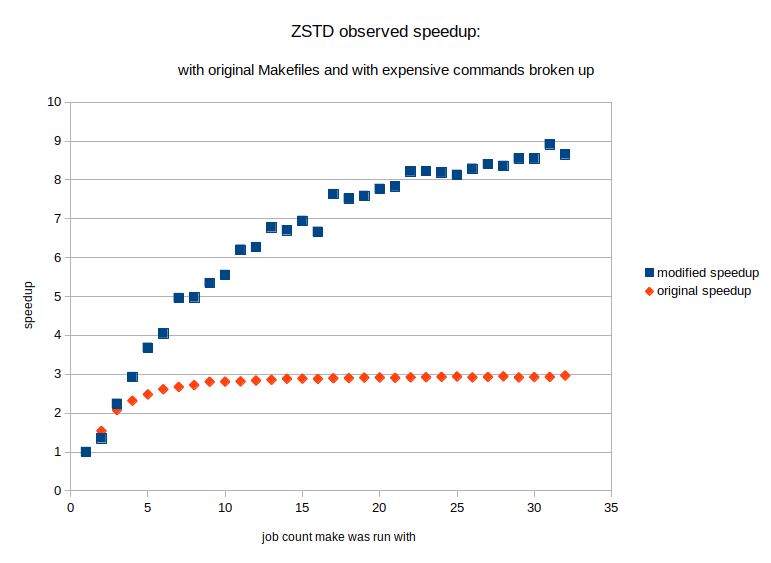
\includegraphics[width=0.5\textwidth]{zstd-speedup}
  \caption{todo}
  \label{fig:zstd}
\end{figure}

All build systems which lack the desired parallelism can be characterized as having too great of
a span in relation to their work.  The span in a build system is the longest (in time) series of
tasks that must be executed sequentially.  In some cases the span is not a series of similar length
tasks but is dominated by a single long running task.  In cases like these it is best to point the
user to the most expensive task in the span because reducing the running time of that task is the
best way to increase the parallelism of the build.

Reducing the running time of non-span tasks will not decrease the running time of the project as
a whole.

To diagnose this problem the user can use the tool to discover the span path through the build
graph and see which target and shell commands are the most time intensive.  The user can then see
what sort of improvement would occur to the span if they were able to decrease the running
time of any target in the graph.  This is useful in the case where decreasing the running time
of a single task gives the build graph a new span path which is dominated by a different also
long running command that prevents the span of the graph from decreasing.

An example of a project with such a build is Facebook's zstd project \cite{}.  If we use our tool
to analyse the span of zstd's build, we see that the original span is dominated by a single call
to cc.

\begin{Verbatim}[commandchars=\\\{\},codes={\catcode`$=3\catcode`^=7\catcode`_=8},fontsize=\small,numbers=left,xleftmargin=5mm]
  cc \$(FLAGS)
  ../lib/common/debug.c
  ../lib/common/entropy\_common.c
  \textrm{\emph{25 more .c files}}
  zstdcli.o fileio.o bench.o
  datagen.o dibio.o -o zstd
\end{Verbatim}

If this call is no longer part of the span, we find that the new span is similarly dominated by
another single call to cc.

\begin{Verbatim}[commandchars=\\\{\},codes={\catcode`$=3\catcode`^=7\catcode`_=8},fontsize=\small,numbers=left,xleftmargin=5mm]
  cc \$(FLAGS)
  common/debug.c
  common/entropy\_common.c
  \textrm{\emph{28 more .c files}}
  -shared -fPIC -fvisibility=hidden
  -Wl,-soname=libzstd.so.1 -o libzstd.so.1.3.7
\end{Verbatim}

If neither of these calls were members of the build's span, then our tool predicts the span would be
7.2 seconds rather than 39 seconds or 37 seconds.  To test this we manually replaced the first of
these two cc calls with 28 new calls to cc; 27 of those are spent compiling each .c file individually
and the last is to link them all together.  Due to this new organization the 27 .c files can be
compiled in parallel.  Similarly, the second cc call is replace with 28 new calls to cc; 27 of which
compile each .c file individually and the last of which links the object files together.

You can see in figure \ref{fig:zstd} that when we ran the modified build with 1 to 32 jobs we
observed the predicted speedup.  An additional performance improvement that we did not predict was
that the work of the new build would decrease from approximately 120 seconds to approximately 80 seconds.

Each of the generated object files is declared as its own target; so when make considers building
each object file it can check if the file already exists and whether it must be rebuilt.  It turns
out that the object files being built as part of the first long cc command, had already been
previously built by make.  By declaring each object file as its own target and building each one
individually then linking them, make was able to determine it wasn't necessary to build them the
2nd time; so the effect time of the first cc command when from 40 seconds to 2 seconds; only the
time necessary for linking the object files together.

\subsection{Bad OS Scaling}

\begin{figure}[]
  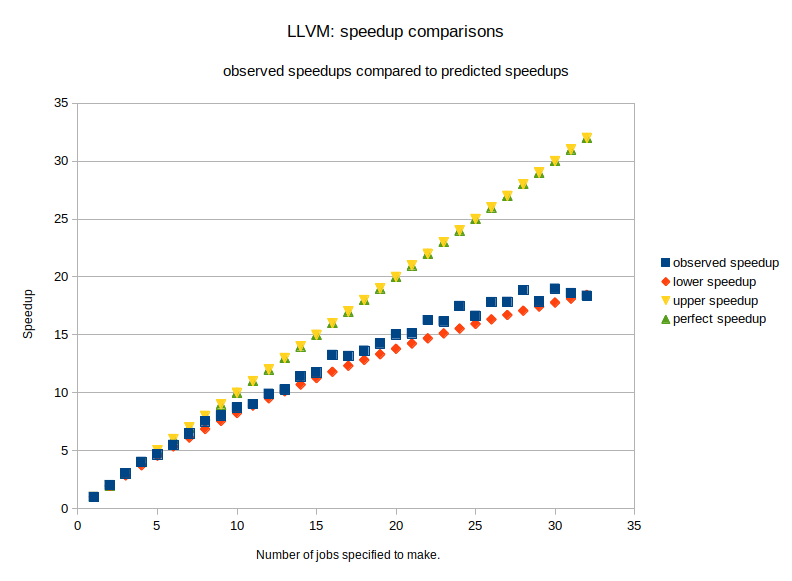
\includegraphics[width=0.5\textwidth]{llvm-speedup}
  \caption{todo}
  \label{fig:llvm}
\end{figure}

Some projects may exhibit ample potential parallelism, but even when run with more threads than
available parallelism, predicted parallelism may not be achieved.  LLVM \cite{} is the largest
project we analysed with a calculated work of approximately 12584 seconds, or 3.5 hours.  The
predicted span of LLVM is 305 seconds, or 5 minutes.  This gives LLVM a parallelism of about 41.
These calculations where made from a build of LLVM that was done not using strace.

A parallelism of 41 would lead one to believe that on a machine with 32 cores LLVM should be built
in parallel in about 5 minutes.  Our observations did not match this expectation.  When LLVM was
built with ``-j 32'' the observed speedup was slightly over 18; see chart \ref{}.  Using work and
span our tool can predict the potential speedup a build will experience using Brent's theorem
\cite{}.  The lower speedup bound is predicted using Brent's theorem, which specifies that for
P processors, \begin{math} T_P \leq T \end{math}

% say something about brent's theorem
% say something about why llvm doesnt achieve the predicted speedup

% project example is LLVM:
% say something about how LLVM is a very large project and 

\subsection{Slow compiler}

A similar issue to the one described in section \ref{sec:expensive} is when a build's
span is dominated by the compilation of a single file.  This problem however cannot be
solved in the makefile like the zstd issue was.  Solutions to this problem include
breaking the file up into smaller files which can be compiled in parallel and then
linked; or changing the compiler so that it is capable of compiling the file faster.
A faster compiler, would have the additional benefit of not only decreasing the span
of the project but also likely decreasing the work of the project.

Google's protocol buffers project \cite{} exhibited this behavior.  It had a relatively
long predicted span of ?? seconds, which was dominated by a call to g++ which was
compiling a single file.  When we apply the same analysis as we applied to zstd in
section \ref{sec:expensive}, we see that if \ref{} wasn't a part of the span, the new
span would be ?? and would be dominated by another g++ compilation of a single file.
And we continue this again to find that the 3 top span paths are dominated by g++
compilations of individual files.  If none of these calls were part of the span, the
new span of the project would be ??.  Now if the developers of protocol buffers were
interested in increasing the parallelism of their project they would know where they
should focus their efforts

Here is a simplification of the real command run by make; it took about 40 seconds to run.
\begin{Verbatim}[commandchars=\\\{\},codes={\catcode`$=3\catcode`^=7\catcode`_=8},fontsize=\small,numbers=left,xleftmargin=5mm]
  g++ \$(FLAGS)
  -o google/protobuf/descriptor.lo
  google/protobuf/descriptor.cc
\end{Verbatim}

Here is a simplification of the real command run by make; it took about 27 seconds to run.
\begin{Verbatim}[commandchars=\\\{\},codes={\catcode`$=3\catcode`^=7\catcode`_=8},fontsize=\small,numbers=left,xleftmargin=5mm]
  g++ \$(FLAGS)
  -o google/protobuf/descriptor.pb.lo
  google/protobuf/descriptor.pb.cc
\end{Verbatim}

Here is a simplification of the real command run by make; it took about 22.5 seconds to run.
\begin{Verbatim}[commandchars=\\\{\},codes={\catcode`$=3\catcode`^=7\catcode`_=8},fontsize=\small,numbers=left,xleftmargin=5mm]
  g++ \$(FLAGS)
  -o google/protobuf/compiler/cpp/cpp\_message.lo
  google/protobuf/compiler/cpp/cpp\_message.cc
\end{Verbatim}

% so, if the problem is with compiling a single file, then we don't really have a
% make level solution to that problem
% user needs to do some work at the file/compiler level to create a solution
% potential solutions include breaking the file up into smaller files which can be
% compiled and linked in paralle
% using a faster compiler, which would have the added benefit of likely decreasing
% the overall work of the build as well as the span
% maybe trying to motivate some future work here

% example project is protobufs c++ version;
% We perform the same analysis that we did in section expensive;
% look at the top spans and what they are dominated by
% we see that the top 3? are dominated by g++ compilations of single files
% and if those are no longer part of the span we half our span; which would result in a
% double speedup
% so we now have a place to focus our energy for improvements
% HIgh level; non make level fix; expensive section is a make level fix; should mention that
% there maybe

\section{Future work}

One of the limitations of this work is that currenlty to collect the necessary data to rebuild
the build graph, the project must be built using a single thread.  This is a burden for projects
that are very long running such as LLVM.  Additionally, building with strace causes an additional
slowdown and inflates the running time of each shell command, which makes the raw numbers
reported by a build graph created with strace on, inaccurate.  In the future for performance sake
it would be good to collect the necessary information while allowing make to run in parallel with
any number of processes.

In addition to this, we hope to analyse more project builds and introduce parallelism at other
level of project builds, such as at the level of the compiler.  

\end{document}
